\chapter{State-of-the-Art}
\label{chapter2}
\hspace*{6mm}To comprehensively contemplate requirements of an endodontic robot such as workspace, payload, clinical problems, works of literature in the dental field are involved. Recent literatures have revealed that researchers have seen the use of dental robot \cite{rawtiya2014application}\cite{s21103308}\cite{bhat2017robotics}, Most largely, implant surgery is widely discussed\cite{haidar2017autonomous}\cite{wu2019robotics}. In this chapter, the pieces of literature about dental robots for implant placement and endodontic treatment will be reviewed.
\section{Robotics in Dentistry}
\hspace*{6mm}Advancements in robot-assisted surgery invigorates researches on robotics in the dental field. However, the majority of robotic applications are in implant surgery. 
\par
The research team in Hong Kong designed a dental manipulator with tendon-sheath mechanism and bracing actuator \cite{Li2019ACD}. The tendon-sheath mechanism drove the whole machine to move and provided flexible manipulations. The soft bracing actuator at the end effector held the handpiece stably due to its stiffness and satisfied the requirement of workspace in a patient mouth. The objective of this robotic system is to perform from operative caries removal, crown preparation, filling, to Orthodontia. However, pre-clinical tasks had not been proven yet.
\begin{figure}[htbp]
\begin{center}
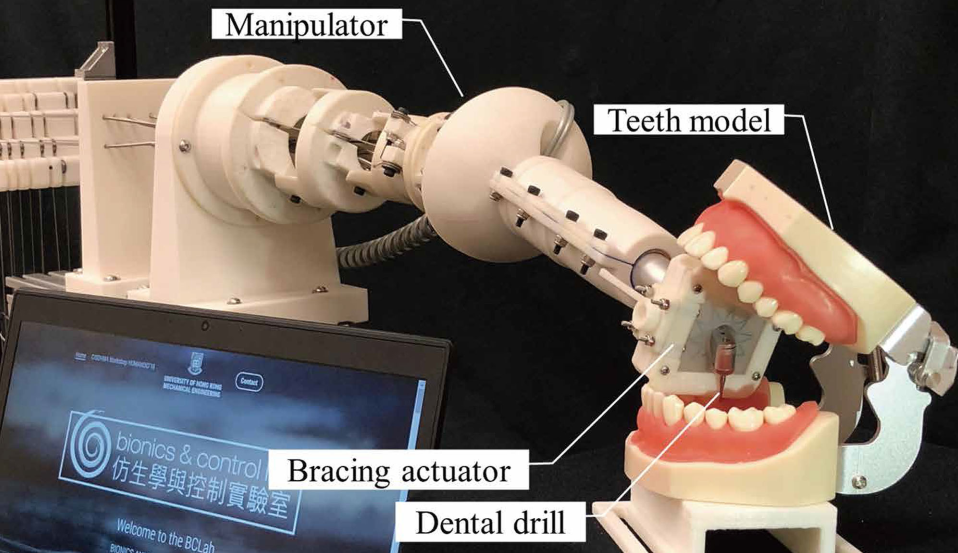
\includegraphics[width=0.9\linewidth]{Images/hongkong_1.png}
\caption[Dental robot designed by the University of Hong Kong]{
Dental robot designed by the University of Hong Kong \cite{Li2019ACD}.
}\label{fig:hongkong}
\end{center}
\end{figure}
\par
G. Kim \textit{et al.} proposed an implant robot based on a double parallelogram mechanism \cite{Kim2009ASO}. The manipulator is shown in Fig \ref{fig:korea}. With the double parallelogram mechanism, the entry point would be constrained at a fixed point and form a remote center of motion (RCM). Besides, a force and torque sensor was integrated to design an admittance type of cooperative manipulator. The manipulator used torque values in the x and y-axis to calibrate the bias caused by drilling. However, it seemed that the prototype of robot did not meet the requirement of dimension and workspace.
\par
T. Iijima \textit{et al.} proposed a master-slave dental system \cite{9026216}. The serial-parallel hybrid mechanism provided remote center of motion (RCM) as shown in Fig \ref{fig:japan}. A reaction force observer (RFOB) was integrated to obtain force information. Acceleration based bilateral control was implemented to communicate master with slave. 
\begin{figure}[htbp]
\begin{center}
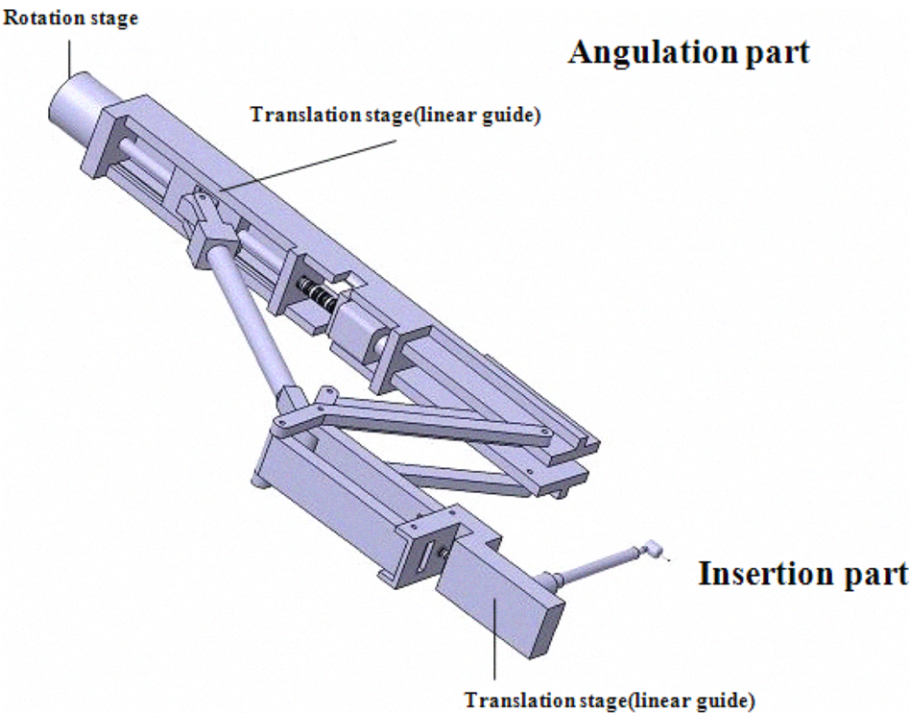
\includegraphics[width=0.7\linewidth]{Images/korea.png}
\caption[Implant robot designed by Chosun university, Korea]{
Implant robot designed by Chosun university, Korea \cite{Kim2009ASO}.
}\label{fig:korea}

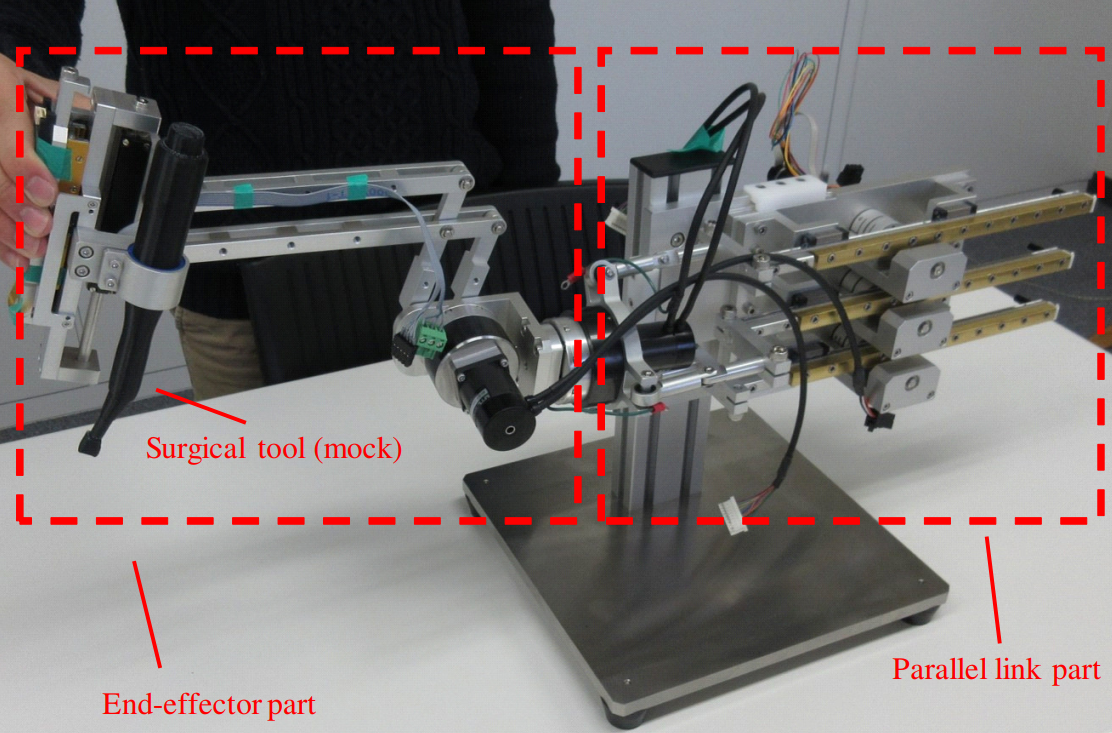
\includegraphics[width=0.7\linewidth]{Images/Japan.png}
\caption[Implant robot designed by Yokohama National University, Japan]{
Implant robot designed by Yokohama National University, Japan \cite{9026216}.
}\label{fig:japan}
\end{center}
\end{figure}

\par
There is a commercial robot, YOMI (Neosis, Miami, Florida, USA) \cite{bolding2021accuracy}\cite{BOLDING2021}, which is a robot-assisted system for minimally invasive implant surgery shown in Fig \ref{fig:YOMI}. YOMI provides precise physical and haptic guidance to perform implant placement because it constrains the drilling position, direction, orientation, and depth. Dentists can design the surgical plan in advance with pre-planning software and adjust it intraoperatively. Undoubtedly it could increase the accuracy of drilling and decrease the surgery time. Also,  once the tool approaches the danger zones such as nerves and sinus cavities, it will alert the dentist to take appropriate measures.
\begin{figure}[htbp]
\begin{center}
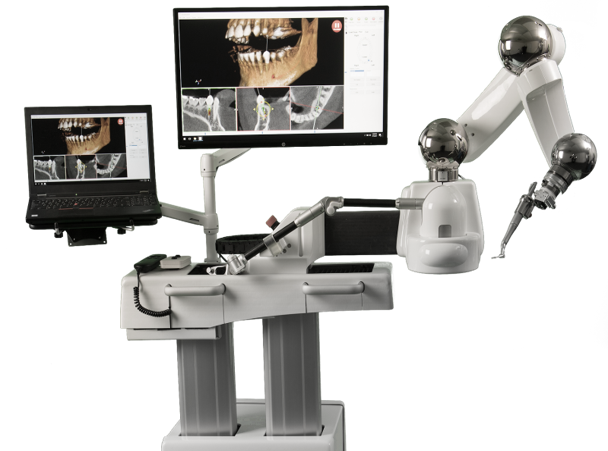
\includegraphics[width=0.8\linewidth]{Images/YOMI.png}
\caption{
Commercial implant robot - YOMI (Neosis, Miami, Florida, USA)
}\label{fig:YOMI}
\end{center}
\end{figure}
\par
An additional robot arm is connected to the intraoral splint which is mounted on patient mouth shown in Fig \ref{fig:patient_tracking}. It enables the robot to keep track of the position information \cite{intraoral_splint} . If the patient moves, YOMI will detect it and alignment immediately to retain the accuracy of the drilling position. Furthermore, it visualizes a 3-D preoperative CT scan and real-time information on the screen to show the updated anatomical features such as drilling entry and bone quantity.  YOMI has received the clearance from FDA and has performed more than $2,700$ surgeries in the USA. In the pandemic of Covid-19 in 2020, YOMI provided non-contact surgery between dentists and patients due to its automatic robotic system. 
\begin{figure}[htbp]
\begin{center}
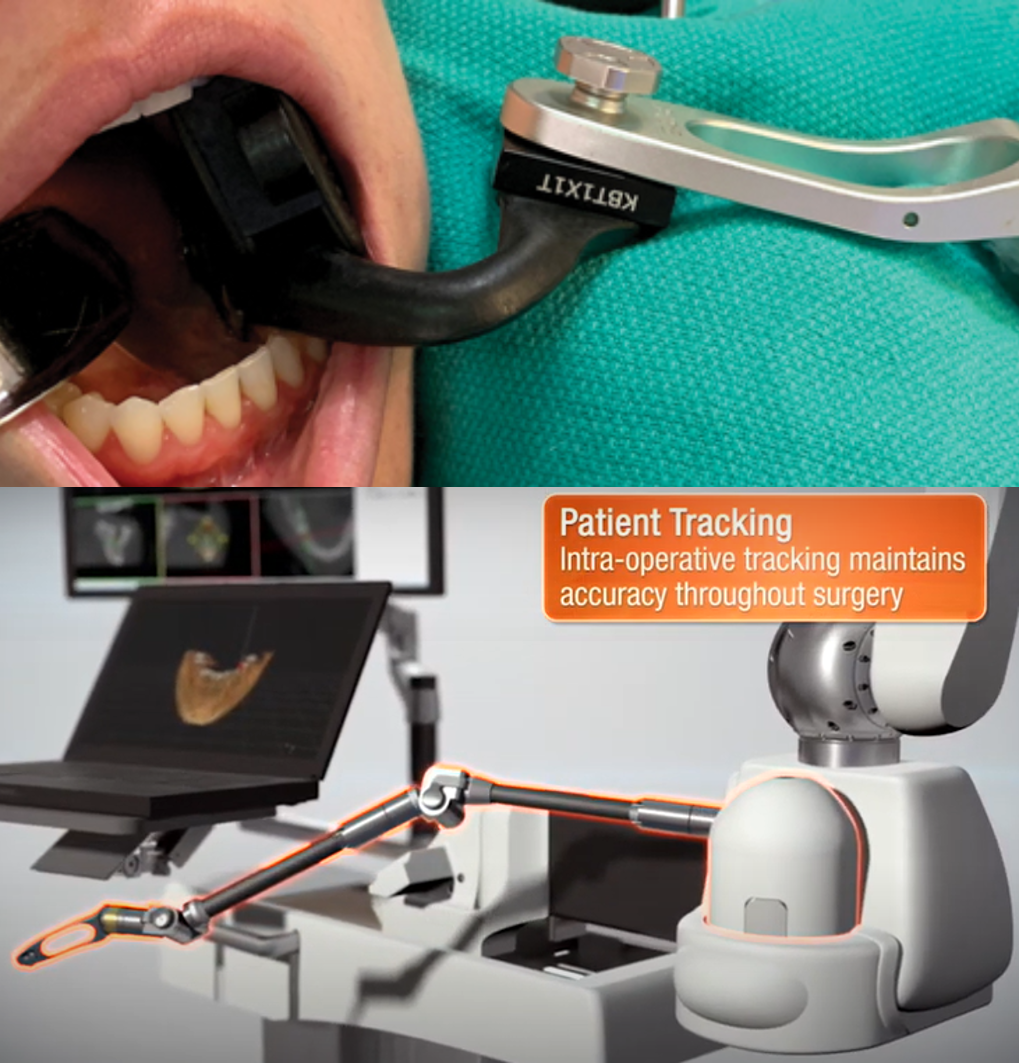
\includegraphics[width=0.8\linewidth]{Images/patient_tracking.png}
\caption[Patient tracking system]{
Patient tracking system \cite{web3}\cite{intraoral_splint}. 
}\label{fig:patient_tracking}
\end{center}
\end{figure}
\section{Endodontic Treatment Robot}
\hspace*{6mm}Endodontic treatment requires a higher precision and accuracy than implant placement. There was a domestic team dedicating to develop an endodontic robot. In Intelligent Micro Robot Development for Minimum Invasive Endodontic Treatment \cite{dong2006wip}\cite{everett2014feasibility}\cite{dong2010design}, their team proposed a complete project, which involves whole endodontic treatment including "Opening", "Cleaning", and "Filling". 
\begin{figure}[htbp]
	\begin{center}
	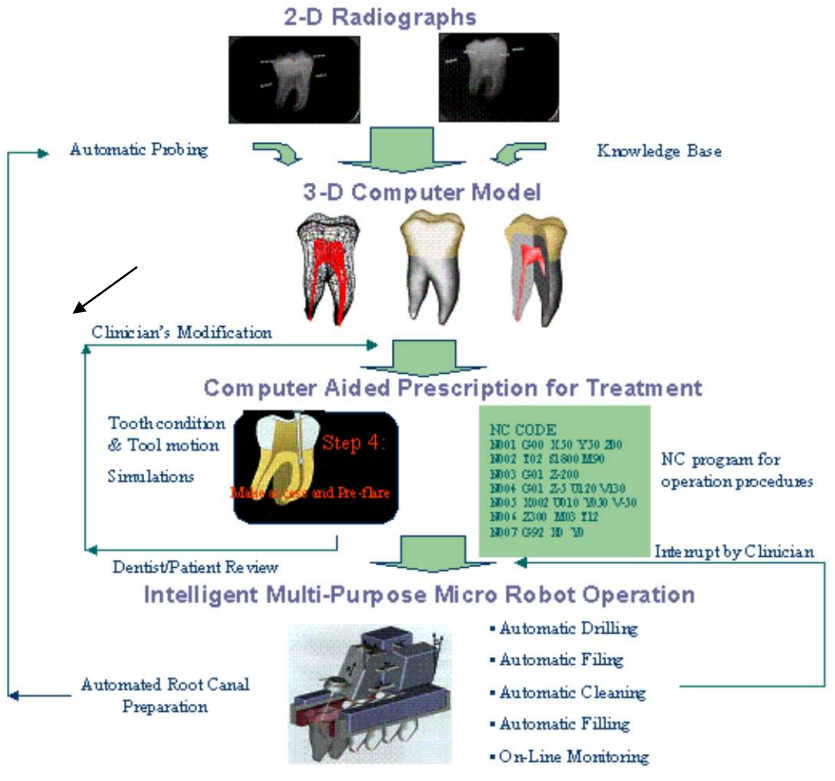
\includegraphics[width=0.95\linewidth]{Images/NCTU_2.png}
	\caption[Project of Micro robot for endodontic treatment proposed by professor Janet Dong]{Project of Micro robot for endodontic treatment proposed by professor Janet Dong \cite{everett2014feasibility}}	
	\label{fig:NCTU_2}
	\end{center}
\end{figure}
\par
The aim of this project was taken apart of several parts as shown in Fig \ref{fig:NCTU_2}. Before starting surgery, it utilized a 2-D X-ray image to build a 3-D computational model and designed the corresponding surgical path by computer-aided treatment procedure planning which is widely used in industry. Intraoperatively a micro-machine with a tool change mechanism was built to drill and fill. Then, an ultrasonic cleaning tool was interfaced to remove the cutting chips and pulps. However, the study using a 2-D X-ray image to build a 3-D model belongs to pre-operation. Any accident during surgery would destroy the ideal pre-planed path.
\par
Also, a micro robot was developed to perform root canal treatment. It was small enough to be mounted on several teeth within a mouth as shown in Fig \ref{fig:NCTU_4}. Therefore, it reduced the patient's inconvenience because it allowed the patient to close their mouth during the surgery.
\begin{figure}[htbp]
\begin{center}
	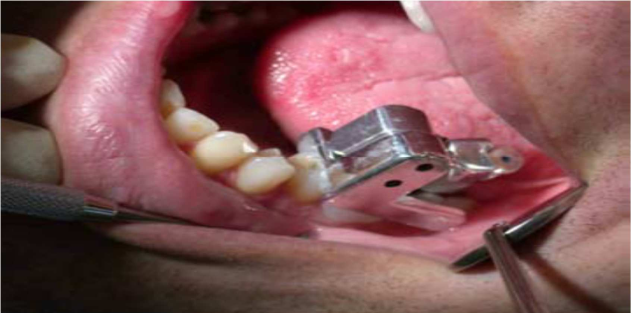
\includegraphics[width=0.9\linewidth]{Images/NCTU_4.png}
	\caption[Endodontic Micro Robot]{Endodontic Micro Robot \cite{dong2006wip}}	
	\label{fig:NCTU_4}
\end{center}
\end{figure}
\begin{figure}[htbp]
\begin{center}
	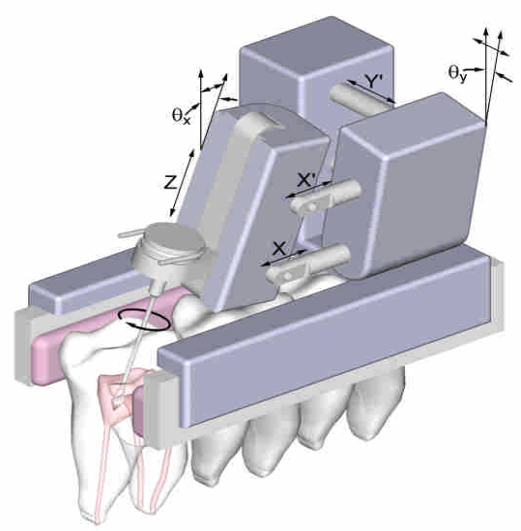
\includegraphics[width=0.6\linewidth]{Images/NCTU_1.png}
	\caption[Multi-purpose micro-machine for automatic endodontic treatment]{
Multi-purpose micro-machine for automatic endodontic treatment \cite{dong2006wip}
}\label{fig:NCTU_1}
\end{center}
\end{figure}
\par
A multi-purpose micro-machine was designed for automatic endodontic treatment as shown in Fig \ref{fig:NCTU_1}. A parallel bracket was installed on the teeth and the micro-machine was mounted on it. There were three radiopaque reference points inside the bracket. The patient with brackets was taken CT scan, and then three radiopaque points were obtained. With three points, a reference frame was built. Therefore, The machine mounted on bracket would recognize the infected tooth. The micro-machine had 6-DoF including five axes and a drilling tool, they were driven by micro actuators.

\begin{figure}[htbp]
\begin{center}
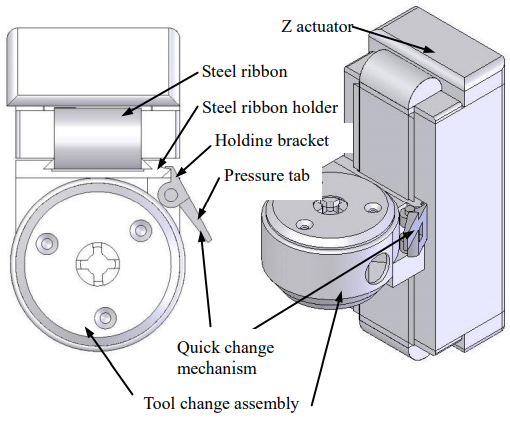
\includegraphics[width=0.7\linewidth]{Images/NCTU_3.png}
\caption[Z-axis actuator with tool change mechanism.]{
Z-axis actuator with tool change mechanism. \cite{dong2010design}
}\label{fig:NCTU_3}
\end{center}
\end{figure}
\par
A tool change mechanism was illustrated in Fig \ref{fig:NCTU_3}. Because there were several procedures during surgery and different tools were used in different phrase. If the machine can hold all types of tools without calibration, the surgery time would decrease dramatically.  Moreover, a hydraulic system was integrated to provide enough drilling force for "Opening" procedure.
\par
However, despite that using 2-D or 3-D image is a appropriate approach to design a surgical path, it belongs to pre-operation. There are many factors to disrupt the surgical path such as uncertain tooth condition and image error. It is not easy to reschedule the motion planning because the root canal in a tooth is unseen by a camera from any angle. Besides, once an endodontic file enters into a root canal, it is hard to obtain the tool tip position due to its flexibility. 
